%%%%%%%%%%%%%%%%%%%%% chapter.tex %%%%%%%%%%%%%%%%%%%%%%%%%%%%%%%%%
%
% sample chapter
%
% Use this file as a template for your own input.
%
%%%%%%%%%%%%%%%%%%%%%%%% Springer-Verlag %%%%%%%%%%%%%%%%%%%%%%%%%%

%%%%%%%%%%%%%%%%%%%%%%%%%%
% CHAPTER 1
%%%%%%%%%%%%%%%%%%%%%%%%%%

%\motto{Use the template \emph{chapter.tex} to style the various elements of your chapter content.}
\chapter{Introduction to project}
\label{intro} % Always give a unique label
% use \chaptermark{}
% to alter or adjust the chapter heading in the running head

\textit{Topics: Novel Nature-Inspired Selection Strategies for Digital Image Evolution of Artwork }

\textit{Genetic programming (GP) is a method used in artificial intelligence to evolve programs suited for a specific job from a population of unfit (often random) programs by applying procedures that resemble natural genetic processes on the population of programs.

The processes comprise choosing the most effective programs for
crossover reproduction and mutation based on a predetermined fitness metric, often competence at the target activity. To create fresh and distinct children that become a part of the future generation of programs, the crossover process includes switching random components of chosen couples (parents). Mutation is the process of replacing one random component of a program with another random component. The next generation replicates certain current generation programs that were not selected for reproduction.

The average member of each new generation is generally more physically fit than the average member of the preceding generation, and the generation\textquotesingle s top programs frequently surpass the generation\textquotesingle s best programs.

When an individual program reaches a specific level of competence or fitness, evolution is typically stopped.

It is possible that a particular run of the algorithm results in a premature conversion to a local maximum, which is not a globally perfect or even desirable outcome.

In order to get a really excellent result, it typically takes multiple runs (dozens to hundreds). To reduce pathologies, it could also be important to start with a big starting population and a wide range of individuals.

Using a finite list of semi transparent polygons, each consisting of a finite number of points, and started with random colour and coordinates, gorgeous paintings may be estimated with astonishingly splendid quality. Polygons develop by changing their colour and coordinates periodically until the resulting mutant meets certain selection criteria for the following generation. Finally, given the limitation that the number of polygons and points per polygon are restricted, a decent approximation of the provided image is obtained.}


%%%%%%%%%%%%%%%%%%%%%%%%%%
% CHAPTER 2
%%%%%%%%%%%%%%%%%%%%%%%%%%

\chapter{Motivation}
\label{Motivation}
{Since machine learning (ML) may be able to address some problems that are too complicated to be handled traditionally, this project captured our interest.

The Simulated Annealing technique is used in machine learning to find the best (or most foretelling) characteristics during the feature selection phase. Without having to look at every single conceivable solution, the approach of simulated annealing is used to discover the optimal answer for a global minimum or maximum.

Comparison of metallurgical annealing and simulated annealing 
for feature selection : In terms of feature selection, the arrangement of molecules in the substance is represented by a set of characteristics (metal).

The number of iterations stands for time. As a result, temperature drops as the number of rounds increases.

The difference in predictive performance between the prior iteration and the current one corresponds to the energy shift in the material.

As a stochastic global search optimization process, Simulated Annealing performs well on non-linear objective functions, in contrast to other local search algorithms, which struggle in this situation.

A finite list of translucent polygons, each with a finite number of points and initialized with random colour and coordinates, can mimic beautiful paintings with amazingly good quality. The polygons change their colour and locations continuously until the mutant meets specific requirements for the following generation. Given the restriction that the number of polygons and the number of points per polygon are limited,
an approximate representation of the provided image is ultimately obtained with excellent precision}


%%%%%%%%%%%%%%%%%%%%%%%%%%
% CHAPTER 3
%%%%%%%%%%%%%%%%%%%%%%%%%%

\chapter{Workflow (Task distribution)}
\label{workflow-task-distribution}
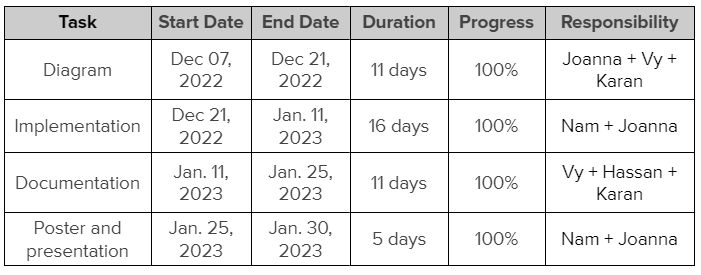
\includegraphics[width=4.5in]{images/Work flow.png}
\break
{
In this project, we decide to go with the sequential workflow. When each
phase is dependent on the completion of the preceding stage, a
sequential workflow exists. If you run a procurement department, for
example, you must wait until the quote is produced and the purchase is
approved before you can pay the invoice. Rule-based workflows containing
conditional logic (e.g., if this, then that) are an example of a
sequential process.
}
\clearpage

%%%%%%%%%%%%%%%%%%%%%%%%%%
% CHAPTER 4
%%%%%%%%%%%%%%%%%%%%%%%%%%
\chapter{Diagrams}
{
In the beginning of the project, we start with the tables of requirement and class diagram. We use class diagrams to model the objects that make up the system, to display the relationships between the objects, and to describe what those objects do and the services that they provide. And final a use case diagram helps us to model the system and user interactions while an activity diagram helps to model the workflow of the system. That is also the reason why we only choose those diagram without drawing 'sequence diagrams' or 'state machine Diagrams' because it don't help much in this project. The project conclude 4 diagrams:
}

{
\centering
1. Table of requirement \\
2. Class diagram \\
3. Activity diagram \\
4. Use-case diagram \\
}
\clearpage

%figure 4.1
\section{Table of requirements}
\begin{figure}
\centering
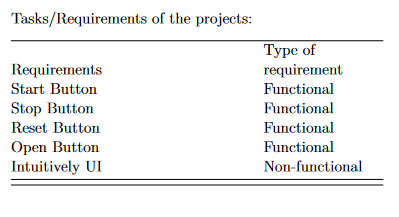
\includegraphics[width=4.5in]{images/taskreqir.png}
\caption{Table of requirements}
\end{figure}

\section{class diagram}
%figure 4.2
\begin{figure}
\centering
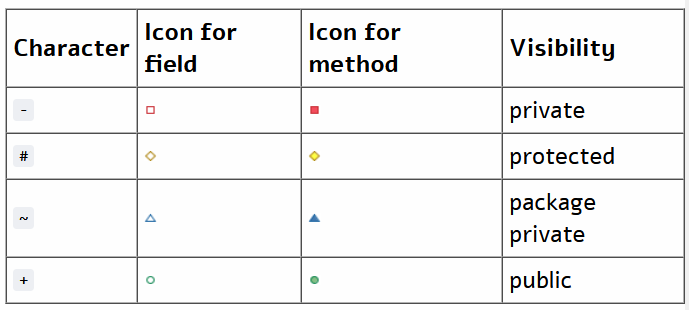
\includegraphics[width=4.5in]{images/image5.png}
\caption{Class Diagram Notation}
\end{figure}


%figure 4.3
\begin{figure}
\centering
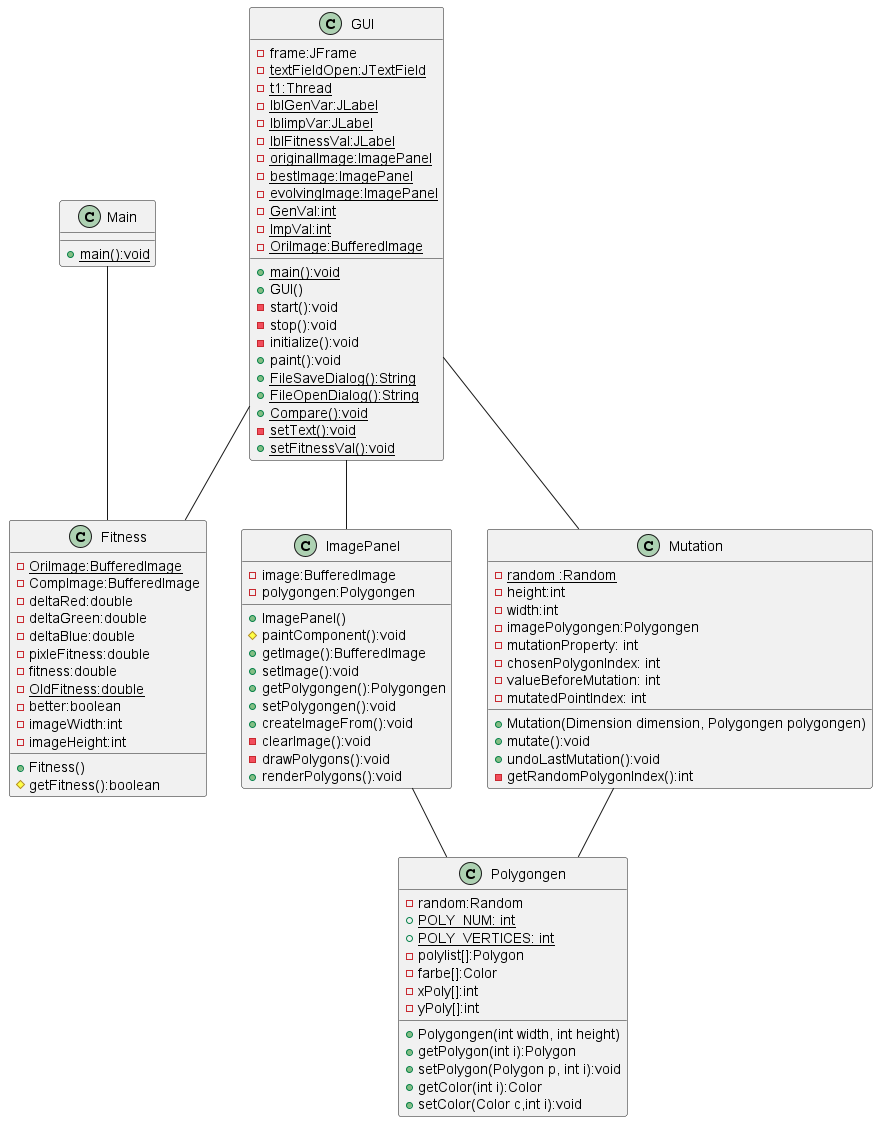
\includegraphics[width=6.3in,height=8in]{images/image12.png}
\caption{Class Diagram}
\end{figure}
\clearpage

\section{Activity diagram}
%figure 4.4
\begin{figure}
\centering
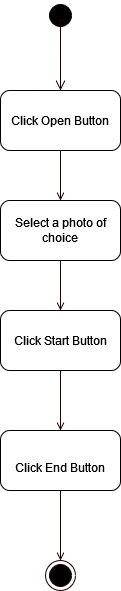
\includegraphics[width=1.3in]{images/image15.png}
\caption{Activity Diagram}
\end{figure}
\clearpage

\section{Use case diagram}
%usecase diagram
\begin{figure}
\centering
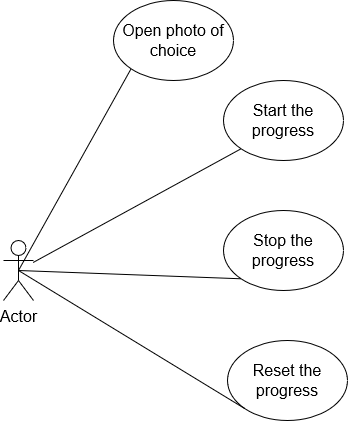
\includegraphics[width=3.0in]{image7.png}
\caption{Use Case Diagram}
\end{figure}
\clearpage

%%%%%%%%%%%%%%%%%%%%%%%%%%
% CHAPTER 5
%%%%%%%%%%%%%%%%%%%%%%%%%%
\chapter{Application preview}
\label{application-preview}
{
A finite list of translucent polygons, each with a finite number of points and initialized with random colour and coordinates, can be used to resemble beautiful paintings with reasonable accuracy. The polygons change their colour and coordinates frequently until the resulting mutation is accepted by some selection criterion for the subsequent generation. Provided the restriction that the number of polygons and the number of points per polygon are limited, an approximate representation of the given image is ultimately obtained with good precision. Below is the main window of the application.
}

\begin{figure}
\centering
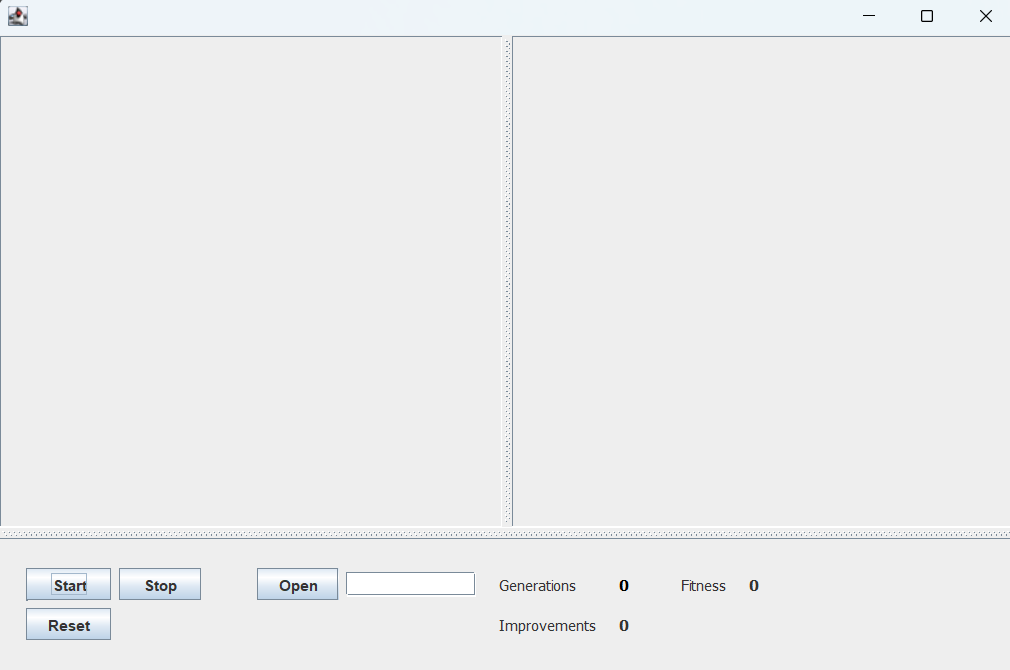
\includegraphics[width=4.5in]{image1.png}
\caption{Application's View}
\end{figure}

{As the user needs a button, add the image first and for that open button is used. When the user clicks on the open button, a located, it will pop up where the user can choose the respective folder where the image is located, which is then uploaded into the system. }

{Below is the user interface of how to choose a folder by clicking on the arrow parallel to look in button.}
\begin{figure}
\centering
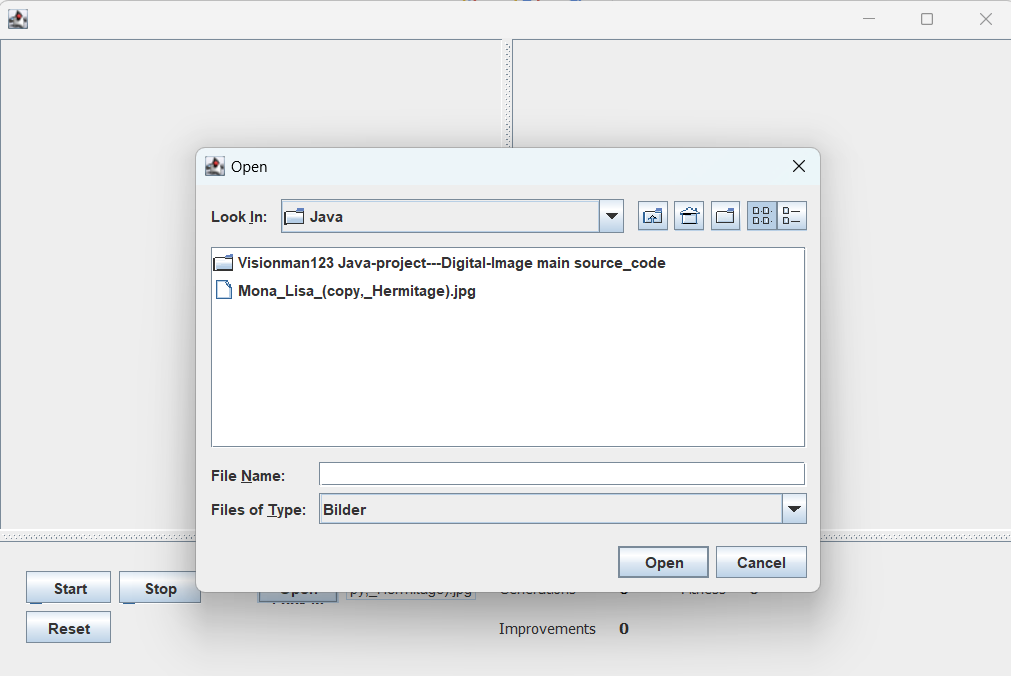
\includegraphics[width=4.5in]{image14.png}
\caption{Application's View}
\end{figure}
\clearpage

{
When the image is already uploaded to the system, user can start the generation by clicking on the start button and with each generation it raises the fitness. The window also provides the information about the number of generations, fitness, and
improvements.
}
\begin{figure}
\centering
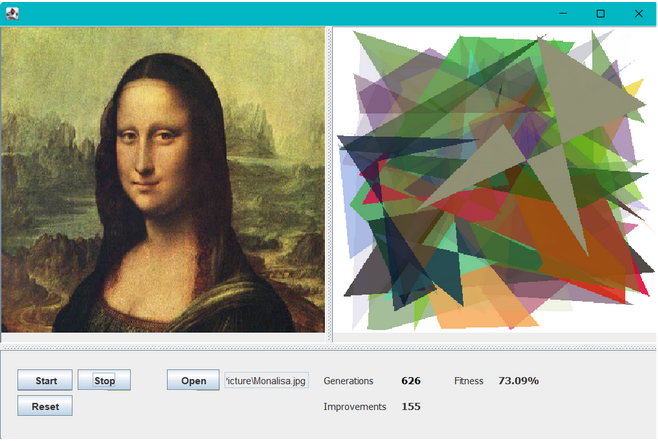
\includegraphics[width=4.5in]{images/5a 1.png}
\caption{Application's View}
\end{figure}
\clearpage


%%%%%%%%%%%%%%%%%%%%%%%%%%
% CHAPTER 6
%%%%%%%%%%%%%%%%%%%%%%%%%%
\chapter{Implementation (Technical Description)}
\label{implementation-technical-description}

% Section
\section{Related works}
\subsection{Genetic programming vs genetic algorithms}
\label{genetic-programming-vs-genetic-algorithms}
Genetic algorithms and genetic programming have many similarities. By evaluating each candidate's fitness among a population of candidates across many generations, they are both used to develop the solution to a problem.

Each generation, new candidates are discovered by randomly modifying (mutation) or swapping pieces of existing candidates (crossover). The candidates that are the least fit are eliminated from the pool.

\subsection{Distinctions in structure}
\label{Distinctions in structure}
The representation of the algorithm or program is the primary
distinction between them.
A set of actions and values---often a string---that makes up a genetic algorithm determines how it is expressed. To understand how to convert for instance a string into a function, a parser must be written for this encoding. Due to the fact that mutation and crossover operations don\textquotesingle t care about the semantics of the method, the parser must also understand how to handle faulty states.To cope with these invalid situations, a strategy must be devised.\\

A tree structure of actions and values, typically a hierarchical data structure, is how a genetic program is expressed. Although a parser must be created for this encoding, genetic programming (mostly) does not result in erroneous states since mutation and crossover operations function inside the tree\textquotesingle s structure.

\subsection{Differences in practice}
\label{Differences in practice}

Using genetic algorithms have a defined length by nature, resulting in limited complexity for the final function. It is necessary to manage invalid situations without causing damage, as they occur frequently. Frequently rely on operator precedence, which is recognized as a restriction in our case when multiplication occurs before subtraction.\\

Genetic programs, which are more flexible since they naturally vary in length, yet they frequently become more complicated. Seldom generates incorrect states, which are frequently dispensable. To completely eliminate operator precedence, use an explicit structure.

% New section
\section{Proposed Approaches}
\label{proposed-approaches}
A finite list of translucent polygons, each with a finite number of points and initialized with random colour and coordinates, can be used to resemble beautiful paintings with reasonable accuracy. The polygons change their colour and coordinates frequently until the resulting mutation is accepted by some selection criterion for the subsequent
generation. Provided the restriction that the number of polygons and the
number of points per polygon are limited, an approximate representation
of the given image is ultimately obtained with good precision.

The application consists of 6 classes to perform a novel nature-inspired
selection strategy for digital image evolution of artwork.
\begin{figure}
\centering
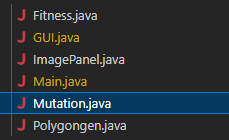
\includegraphics[width=2.4in]{image9.png}
\caption{Java classes}
\end{figure}

\subsection{Polygons}
\label{Polygons}
The Polygons class is responsible for generating random polygons with a specified number of vertices. These polygons are then used as the building blocks for the evolved image. A finite set of n polygons is used. Each polygon is coloured using the ARGB (alpha red green blue) colour system and has a set number of vertexes, m. Each vertex is identified by its x and y coordinates, and the four values a (alpha), r (red), g (green), and b (blue) are used to identify it. All values are stated as integers to assure the accuracy of each element in the solution set, and the entire solution is encoded into a series of numbers that reflect the aforementioned values. This encoding technique for a solution set provides a precise mechanism for representing polygons and their
associated values.
\begin{figure} 
\centering
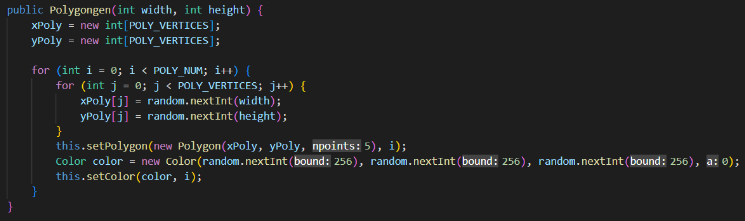
\includegraphics[width=4.5in]{images/polygons 1.png}
\caption{Java classes}
\end{figure}
\clearpage

\subsection{Mutation}
\label{Mutation}
Mutation
The Mutation class is responsible for comparing the randomly generated polygons with the input image and accepting or removing the compared polygons in order to better match the input image. This process is repeated until a fitness match is found.
\begin{figure}
\centering
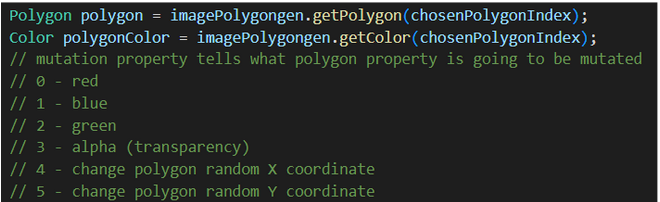
\includegraphics[width=4.5in]{images/polymu.png}

\caption{Mutation class}
\end{figure}
\\
There are three types of mutation possible, which are://

a. Single attribute Mutation: change the value to a random number at a random location in the candidate solution's sequence and beyond a certain threshold, give the new value a random offset.

b. Hill climbing mutation: every iteration, either a vertex attribute or a colour attribute is modified at random.

c. Genetic Mutation: change a random number of attributes 
\\
\\And the genetic mutation also our choices of mutation for evolving picture with undo last Mutation:

\begin{figure}
\centering
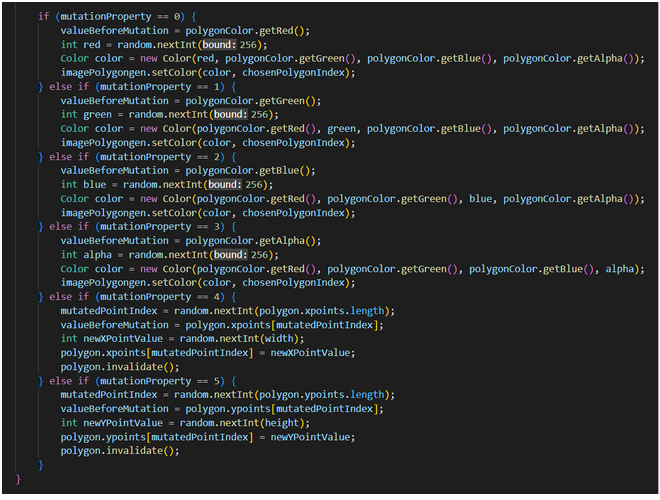
\includegraphics[width=4.5in]{images/elseif.png}
\caption{Mutation class 2}
\end{figure}

\\

\\

\begin{figure}
\centering
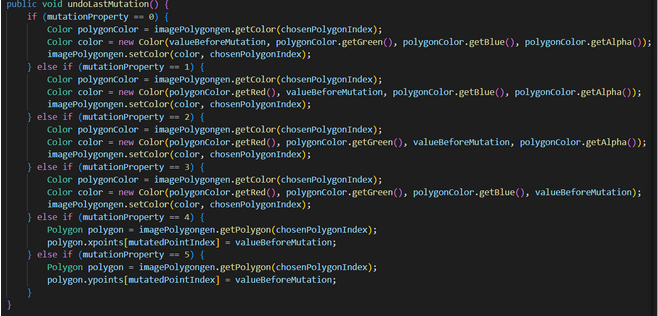
\includegraphics[width=4.5in]{images/undomu.png}
\caption{undoLastMutation function}
\end{figure}
\newpage


\subsection{Fitness class}
\label{Fitness class}

The Fitness class is responsible for comparing the randomly generated polygons with the input image and determining the similarity between them. 
\begin{figure}
\centering
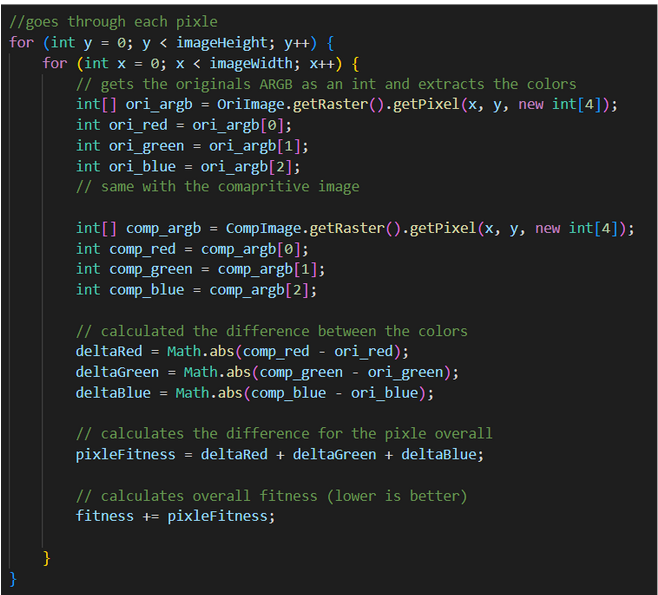
\includegraphics[width=4.5in]{images/fitness.png}

\caption{Fitness class }
\end{figure}

\newpage
This allows the program to identify which polygons best match the input image. A byte-to-byte mapping between a candidate solution and the desired result is carried out by the fitness function.

\begin{figure}
\centering
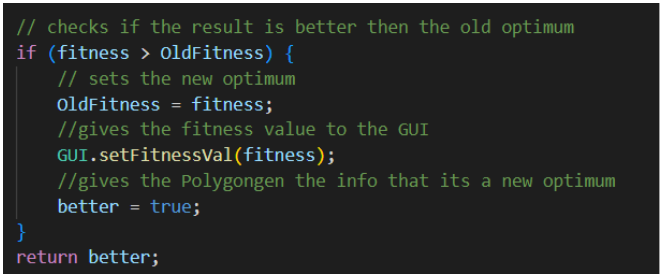
\includegraphics[width=4.5in]{images/fitness2.png}
\caption{Fitness class 2}
\end{figure}
\newpage


\subsection{Image Panel}
\label{Image Panel}
The Image Panel class is responsible for displaying the input image and the evolved image. 

\begin{figure}
\centering
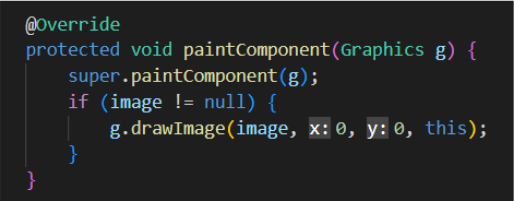
\includegraphics[width=4.5in]{images/impa.png}

\caption{Image Panel class}
\end{figure}
This allows the user to see the progress of the evolution process and compare the two images.
\begin{figure}
\centering
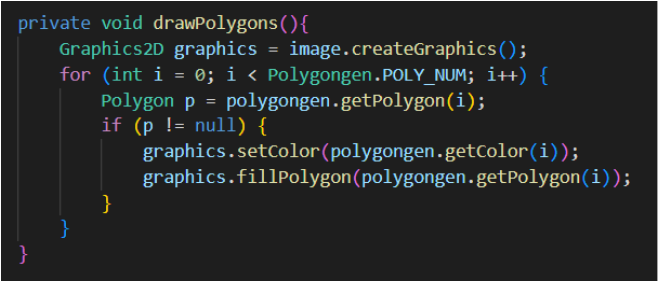
\includegraphics[width=4.5in]{images/impa2.png}

\caption{Image Panel class 2}
\end{figure}
\newpage

\subsection{GUI class }
\label{GUI class}
The GUI class produces the user interface, which allows the user to upload the image and to start and stop the evolution process with the help of buttons.

The  Open Button is using to implement the open file action, it allows user to add their picture from their library


\begin{figure}
\centering
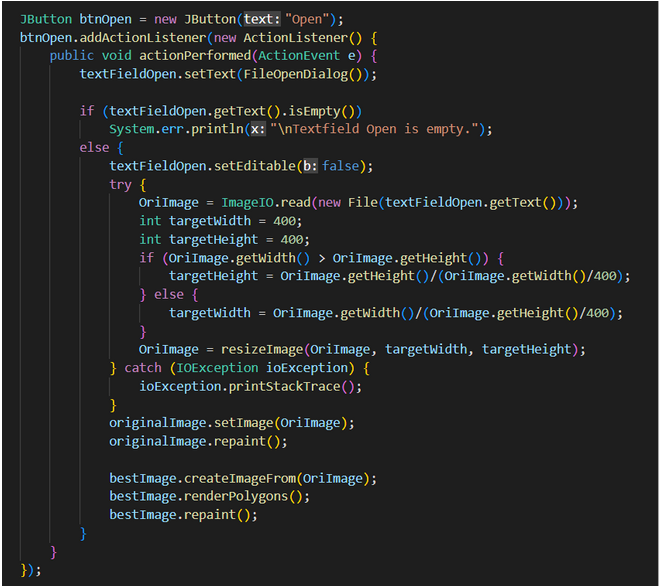
\includegraphics[width=4.5in]{images/gui.png}

\caption{GUI 1}
\end{figure}
\newpage

Which connect directly to the FileOpenDialog and FileSaveDialog. 
\begin{figure}
\centering
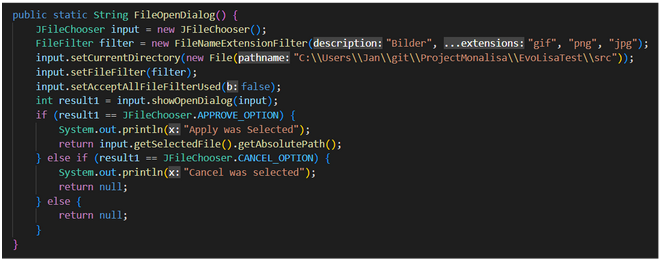
\includegraphics[width=4.5in]{images/gui2.png}
\caption{GUI 2}
\end{figure}

To avoid users selecting the wrong file which leads to the system failure. The filter for files has been added, it only allow the file in format gif, png, jpg 
\begin{figure}
\centering
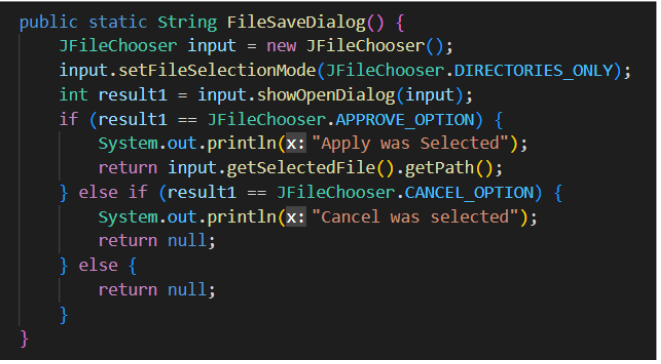
\includegraphics[width=4.5in]{images/gui3.png}
\caption{GUI 3}
\end{figure}

\newpage

The start, stop, reset button using for drawing the lecture

\begin{figure}
\centering
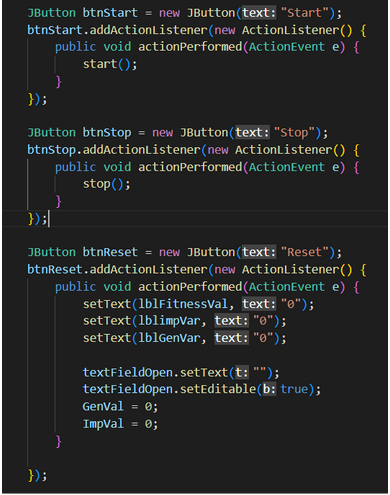
\includegraphics[width=4.5in]{images/gui4.png}

\caption{GUI 4}
\end{figure}
\newpage
The resizePicture function is using for avoid user adding large/small scale image, so that it will resize all the picture into 400x400 pixel 

\begin{figure}
\centering
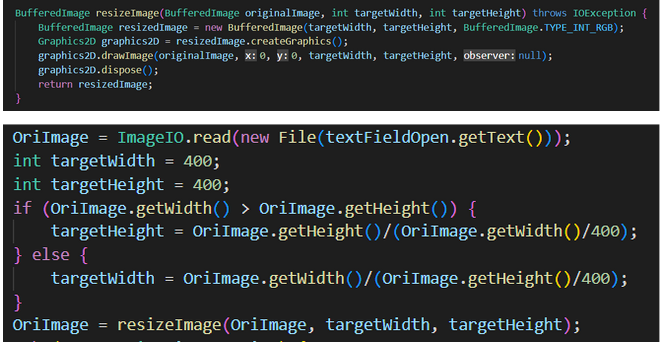
\includegraphics[width=4.5in]{images/gui5.png}

\caption{GUI 5}
\end{figure}
Finally, the Main class ties everything together and runs the program. It creates instances of the other classes and coordinates their interactions to perform the image evolution process
\begin{figure}
\centering
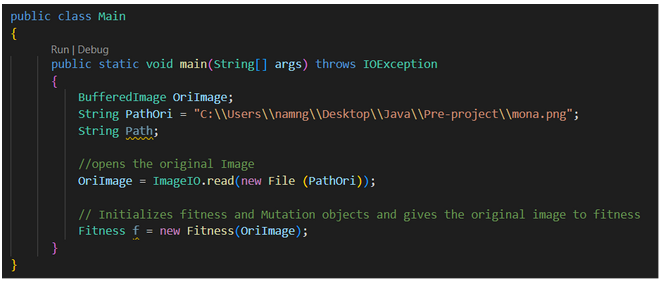
\includegraphics[width=4.5in]{images/main.png}

\caption{Main}
\end{figure}


\section{GUI Design}\label{GUI Design}
Wireframes 1 - Problem: Introduction page: Short brief about the Digital Image. We using balsamiq wireframes to draw a draft overview about the GUI before coding by Java swing
\begin{figure}
\centering
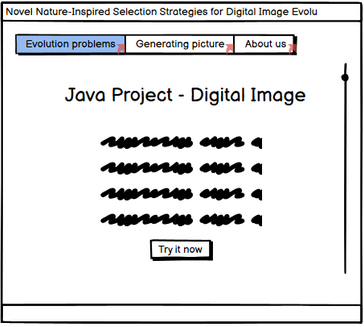
\includegraphics[width=4.5in]{images/wf1.png}
\caption{Wireframes 1 Introduction page}
\end{figure}
\newpage

Wireframes 2 - Generating: Here you can start running with the default image (Monalisa), you can also control the Mutation and Initialize DNA as you want.
\begin{figure}
\centering
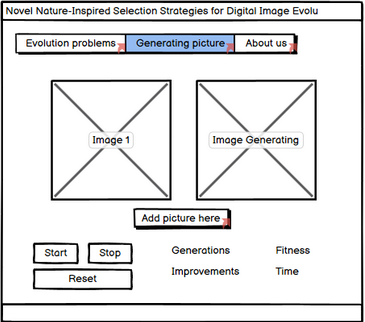
\includegraphics[width=4.5in]{images/wf2.png}
\caption{Wireframes 2 - Generating}
\end{figure}
\newpage

 Wireframes 3 - Add picture: This will pop up after you click the button “Add your image here”. Beside the Monalisa pictures, you can also choose some pictures we already add into our library or you can also add new pictures from your desktop → after you click done, it will return back to the “Wireframes 2 - Generating”
\begin{figure}
\centering
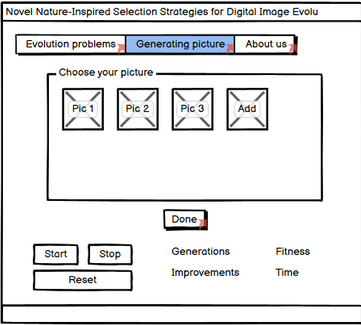
\includegraphics[width=5in,height=4in]{images/wf3.png}
\caption{Wireframes 3 - Add picture}
\end{figure}
\newpage

Wireframes 4 - About us: Like others websites, we also include this (School, MatricNumber, Pictures, Name, Emails to contact if the readers have questions). At the end we also add the github link + report link
\begin{figure}
\centering
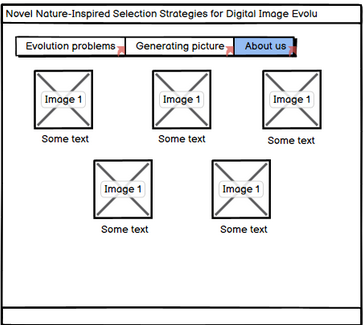
\includegraphics[width=5in,height=4in]{images/wf4.png}
\caption{Wireframes 4 - About us}
\end{figure}

Note: Because we only have a few weeks developing the GUI, we have problems in linking elements between screens and we don't have enough time to fix those bugs. So we decided to only make Wireframe 2 in this project. We plan to develop it more in the future.
\clearpage


\section{GUI Details}
\label{gui-details}

The GUI, or graphical user interface, created with the Java Swing framework. The GUI's objective was to offer a simple and easy-to-use user interface for communicating with the  platform.
Below the UI is explained in detail with the help of screenshots.

\begin{figure}
\centering
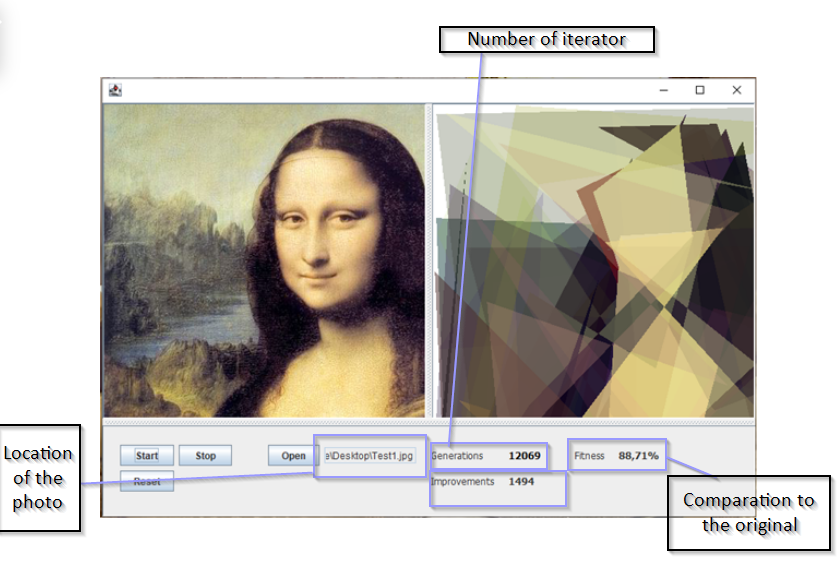
\includegraphics[width=4.5in]{image8.png}
\caption{GUI Details}
\end{figure}
\newpage

\section{JFC/Java Swing}
\label{jfcjava-swing}
A Java-based framework called Java Swing is used to build graphical user interfaces (GUIs) for Java applications. It offers a wide variety of editable elements that may be used to build dynamic, interactive user interfaces, including buttons, labels, text fields, tables, and more. Swing is a potent tool for developing responsive and interactive user interfaces, since it is intended to be platform-independent and event-driven. It is a common option for Java developers and is commonly employed in the creation of desktop applications.\\
Because of its extensive selection of widgets, adaptable look and feel, and multi-threading capability, the Java Swing framework was chosen. Our program can operate on various platforms because of Swing's cross-platform compatibility, which eliminates the need for platform-specific code.\\
The Java Swing framework offered a complete and advanced set of tools for developing the GUI for our system, in conclusion. We were able to design a simple and user-friendly interface thanks to its extensive widget library and layout management features.\\
A class which contains another class is called a container class and for creating GUI at least one container class is compulsory.\\
 Below are the three types of container classes given.
\begin{enumerate}
\item Panel – It is used to organize components on to a window
\item Frame – A fully functioning window with icons and titles
\item Dialogue – It is like a pop-up window but not fully functional like the frame
\end{enumerate}

\begin{figure}
\centering
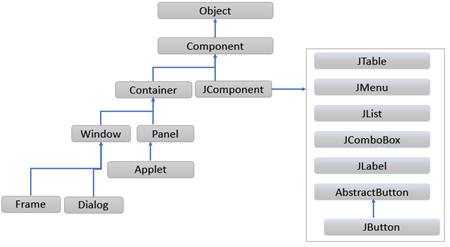
\includegraphics[width=4.5in]{images/java-swing-class-hiearchy.png}
\caption{JFC/Java Swing class hierarchy}
\end{figure}
\clearpage

%%%%%%%%%%%%%%%%%%%%%%%%%%
% CHAPTER 7
%%%%%%%%%%%%%%%%%%%%%%%%%%
\chapter{Experimental Results and Statistical Test}
\label{experimental-results-and-statistical-test}

\textit{
In this section we created a small program that keeps a string of DNA for polygon rendering.
The procedure of the program is quite simple:\\
1. Setup a random DNA string  (application start)\\
2. Copy the current DNA sequence and mutate it slightly\\
3. Use the new DNA to render polygons onto a canvas\\
4. Compare the canvas to the source image\\
5. If the new painting looks more like the source image than the previous painting did, then overwrite the current DNA with the new DNA\\
6. Repeat from 1\\

We start to run the code with three picture "Monalisa", "Pokemon" and "The Starry Night" and receive the result below
} 
\clearpage

\section{Monalisa}
\begin{figure}
\centering
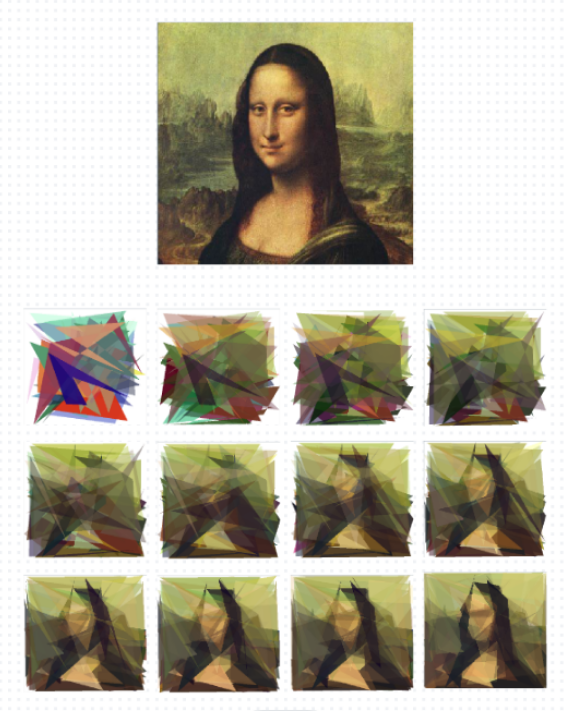
\includegraphics[width=4.5in]{images/7a 1.png}
\caption{Monalisa}
\end{figure}
\clearpage

\section{Pokemon}
\begin{figure}
\centering
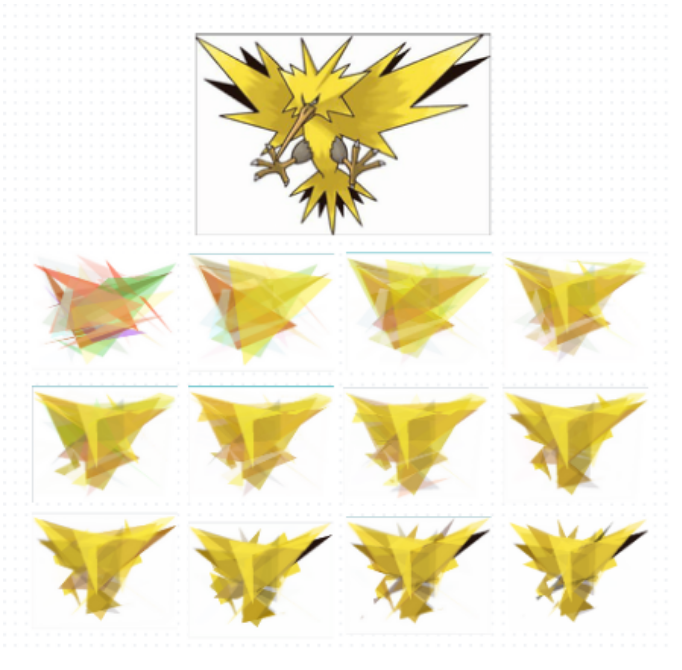
\includegraphics[width=5in,height=6in]{images/7a 2.png}
\caption{Pokemon}
\end{figure}
\clearpage

\section{The Starry Night}
\begin{figure}
\centering
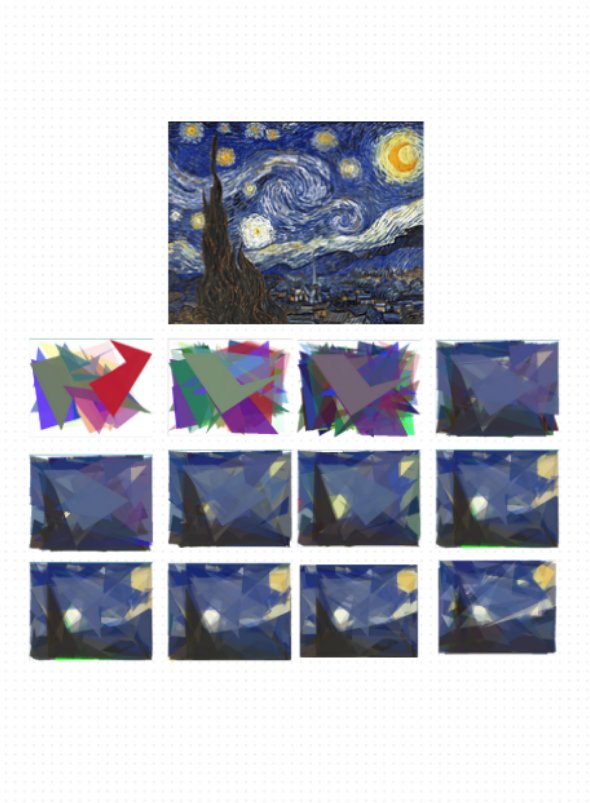
\includegraphics[width=5in,height=6in]{images/7a 3.png}
\caption{The Starry Night}
\end{figure}
\clearpage

%%%%%%%%%%%%%%%%%%%%%%%%%%
% CHAPTER 8
%%%%%%%%%%%%%%%%%%%%%%%%%%
\chapter{Conclusions and Future Work }
\label{conclusions-and-future-work}

\section{What you have learned}
\label{what-you-have-learned}
Our experience with Java so far has been out of the world. We would like to highlight some of the key things which we learned with the help of Java. Java has more built-in features than languages like Python or JavaScript, but since Java is so expressive, these features are simple to find and utilize. A developer has the choice to print text to the output log files, the console screen, or even the Windows dialogue box, even for a basic Hello World application. The vast feature set of Java can be intimidating. However, Java\textquotesingle s expressiveness enables developers to easily access features and functions. Java uses dot notation to connect objects, attributes, and methods in a chain. The majority of other programming languages also do it. The object-oriented syntax of Java will be easy for anyone who is familiar with JavaScript, C++, or Python to learn. Parenthesis are rounded brackets.
Java employs a combination of square, round, and curly brackets. Curly and rounded brackets, however, aren't\textquotesingle t properly called brackets:

Parentheses are denoted by round brackets ().
Braces are indicated by square brackets {[}{]}.
Braces are curved brackets.
Text is enclosed in double quotations.
In HTML and JavaScript, single quotes are the norm. Not in Java. In Java, text Strings go inside double quotes. If one puts text Strings inside single quotes, the code will not compile. Dot notation is used in Java. Java employs dot notation to link objects, properties, and methods together. The majority of other programming languages also do it. The object-oriented syntax of Java will be easy for anyone who is familiar with JavaScript, C++, or Python to learn.

Our initial lack of knowledge about Scrum development and our isolation from one another affected the team\textquotesingle s productivity. Later we stumbled upon Sprint. A scrum team strives to finish a specific amount of work during a brief, time-boxed sprint. Agile teams may provide better software with fewer headaches if sprints are done correctly because they are the foundation of scrum and agile approaches. With scrum, a product is created in a series of sprints that divide large, complex projects into manageable portions.

Agile values and scrum procedures are fairly associated due to their many commonalities. Sprints assist teams in living the agile values of “responding to change over following a plan” and “delivering working software frequently.'' Agile and the idea of sprints are compatible, and the scrum values of transparency, inspection, and adaptation are essential.


\section{Ideas for the future development of your
application, new algorithms
}
\label{ideas-for-the-future-development-of-your-application-new-algorithms}
The physical annealing process, in which a metal is fully heated and then allowed to cool down gradually, serves as the basis for the simulated annealing optimization technique. In order to modify it to the appropriate shape. When viewed through the lens of machine learning, this approach is a probabilistic optimization strategy that may be used to solve problems with numerous local minima.

The program initially considers the entire model and runs with a random value of minimum. The model is then optimized by arbitrarily lowering some of the parameters. Through the use of an annealing schedule, the model is optimized over the course of n iterations in search of the best outcome. 
This optimization technique is extensively used in various problems like the travelling salesman problem, where the main focus is to find a globally optimal solution by iterating through random probabilistic values.

Simulated Annealing Algorithm has an advantage over gradient descent. From a coding standpoint, the Simulated Annealing approach is simpler to use and implement because it doesn't rely on any model-restrictive features. The Simulated Annealing approach is more dependable and robust because it relies on the probabilistic distribution principle, which guarantees that the model finds the best solution for all potential uncertainties and that nonlinear data can be easily integrated.

Some observations on the SLP algorithm :
The SLP algorithm is an easy-to-understand method for resolving restricted optimization issues. It can be used to solve design issues in engineering, particularly those with lots of design variables. The SLP method's advantages and disadvantages are highlighted in the following observations.

1. The technique shouldn't be applied to engineering design issues as a black box solution. It is better to choose move limitations in an interactive manner because it requires some trial and error.

2. Since no descent function is provided and no line search is carried out in the search direction to determine a step size, the approach might not converge to the precise minimum.

3. If the ideal solution is not a vertex of the feasible set, the procedure can alternate between two positions.

4. Both theoretically and numerically, the procedure is very straightforward. In practice, it might be utilized to obtain better designs, even though it might not be able to attain the precise local minimum point with it.

\newpage

%%%%%%%%%%%%%%%%%%%%%%%%%%
% CHAPTER 7
%%%%%%%%%%%%%%%%%%%%%%%%%%
\chapter{References}
\label{References}
%%%%%%%%%%%%%%%%%%%%%%%% referenc.tex %%%%%%%%%%%%%%%%%%%%%%%%%%%%%%
% sample references
% %
% Use this file as a template for your own input.
%
%%%%%%%%%%%%%%%%%%%%%%%% Springer-Verlag %%%%%%%%%%%%%%%%%%%%%%%%%%
%
% BibTeX users please use
% \bibliographystyle{}
% \bibliography{}
%
\begin{thebibliography}


% Online Document
1.\url{https://github.com/peterbraden/genetic-lisa}
\newline
2.\url{https://rogerjohansson.blog/2008/12/07/genetic-programming-evolution-of-mona-lisa/}
\newline
3.\url{https://alteredqualia.com/visualization/evolve/}
\newline
4.\url{shorturl.at/ilyDG}
\newline
5.\url{https://stackoverflow.com/questions/3819977/what-are-the-differences-between-genetic-algorithms-and-genetic programming}
\end{thebibliography}

